\documentclass{article}
\usepackage[utf8]{inputenc}

\usepackage{amsmath}
\usepackage{amssymb}
\usepackage{amsthm}

\usepackage{caption}
\usepackage{graphicx}
\usepackage[top=0.5in, bottom=0.5in, left=1in, right=1in]{geometry}

\usepackage{titlesec}
    \titlespacing{\subsection}{\parindent}{10pt}{10pt}

\usepackage{titling}
    \newcommand{\studentnumber}[1]{\gdef\studentnumber{#1}}
    \renewcommand{\maketitlehookc}{\par \large \centering \studentnumber \vspace{10pt} \par}

\title{Network Science: Assignment 1}
\author{Syed Arham Naqvi}
\studentnumber{100590852}
\date{\today}

\begin{document}

    \maketitle

    \section*{1.}
        \subsection*{a)}
        \begin{figure}[ht] % You can adjust the [ht] placement options
            \centering
            \begin{minipage}[t]{0.5\textwidth}
                \centering
                \captionsetup{labelformat=empty} % Remove the label ("Figure 1:")
                \caption{Graph of $G^{c}$:}
                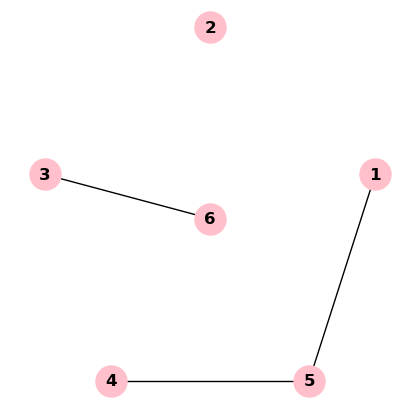
\includegraphics[width=2in]{Gc.png}
            \end{minipage}%
            \begin{minipage}[t]{0.5\textwidth}
                \captionsetup{labelformat=empty} % Remove the label ("Figure 1:")
                \caption{Adjacency Matrix of $G^{c}$:}
                % Matrix goes here
                \[
                \begin{bmatrix}
                    0 & 0 & 0 & 0 & 1 & 0 \\
                    0 & 0 & 0 & 0 & 0 & 0 \\
                    0 & 0 & 0 & 0 & 0 & 1 \\
                    0 & 0 & 0 & 0 & 1 & 0 \\
                    1 & 0 & 0 & 1 & 0 & 0 \\
                    0 & 0 & 1 & 0 & 0& 0 \\
                \end{bmatrix}
                \]
            \end{minipage}
        \end{figure}

        \subsection*{b)}
            \begin{minipage}{1\textwidth}
                If $p$ is the density of $G$ then the density of $G^{c}$ must be
                $1-p$. This is because the amount of nodes remains constant in both graphs
                but $E(G^{c})$ contains all those edges not in $E(G)$.\\

                More formally, let $n=|V(G)|$, we know it also must then be true that $n=|V(G^{c})|$ since the
                number of nodes is the same for both graphs. We can now use $|E(k_{n})|$ where $k_{n}$ is the complete
                graph on $n$ nodes as the denominator for the densities of both $G$ and its complement:
                $$ p= \frac{|E(G)|}{|E(k_{n})|}, \hspace{10pt}p^{c}=\frac{|E(G^{c})|}{|E(k_{n})|}$$
                
                Thus, if $E(G^{c})$ are all those edges not in $E(G)$, then $E(k_{n}) = E(G) \cup E(G^{c})$ and
                $E(G) \cap E(G^{c}) = \emptyset$.\\
                So,
                \begin{align*}
                                         |E(k_{n})| &= |E(G)| + |E(G^{c})|\\
                    \frac{|E(k_{n})|}{|E(k_{n})|} &= \frac{|E(G)|}{|E(k_{n})|} + \frac{|E(G^{c})|}{|E(k_{n})|}\\
                                                1 &= p + p^{c}\\
                                            p^{c} &= 1 - p
                \end{align*}
                $ \therefore $ the density of $G^{c} = 1 - p \qed$
            \end{minipage}
        
    \section*{2.}
        \subsection*{a)}
        \begin{figure}[ht] % You can adjust the [ht] placement options
            \centering
            \begin{minipage}[t]{0.5\textwidth}
                \centering
                \captionsetup{labelformat=empty} % Remove the label ("Figure 1:")
                \caption{Graph of $G$:}
                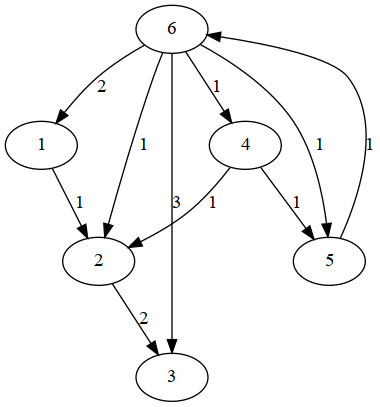
\includegraphics[width=2in]{multi.png}
            \end{minipage}%
            \begin{minipage}[t]{0.5\textwidth}
                \captionsetup{labelformat=empty} % Remove the label ("Figure 1:")
                \caption{Adjacency Matrix of $G$:}
                % Matrix goes here
                \[
                \begin{bmatrix}
                    0 & 1 & 0 & 0 & 0 & 0 \\
                    0 & 0 & 2 & 0 & 0 & 0 \\
                    0 & 0 & 0 & 0 & 0 & 0 \\
                    0 & 1 & 0 & 0 & 1 & 0 \\
                    0 & 0 & 0 & 0 & 0 & 1 \\
                    2 & 1 & 3 & 1 & 1 & 0 \\
                \end{bmatrix}
                \]
            \end{minipage}
        \end{figure}

        \subsection*{b)}
        The only node in $G$ that qualifies as a sink node is node $3$.

        \subsection*{c)}
            \begin{minipage}[t]{1\textwidth}
                $s_{1}^{in} = 2, \hspace{10pt} s_{2}^{in} = 3, \hspace{10pt} s_{3}^{in} = 5, \hspace{10pt} s_{4}^{in} = 1
                , \hspace{10pt} s_{5}^{in} = 2, \hspace{10pt} s_{6}^{in} = 1\\\\
                s_{1}^{out} = 1, \hspace{10pt} s_{2}^{out} = 2, \hspace{10pt} s_{3}^{out} = 0, \hspace{10pt} s_{4}^{out} = 2
                , \hspace{10pt} s_{5}^{out} = 1, \hspace{10pt} s_{6}^{out} = 8
                $
            \end{minipage}

        \subsection*{d)}
            \begin{figure}[ht] % You can adjust the [ht] placement options
                \begin{minipage}[t]{0.5\textwidth}
                    \centering
                    \captionsetup{labelformat=empty} % Remove the label ("Figure 1:")
                    \caption{Undirected, Unweighted Network $H$:}
                    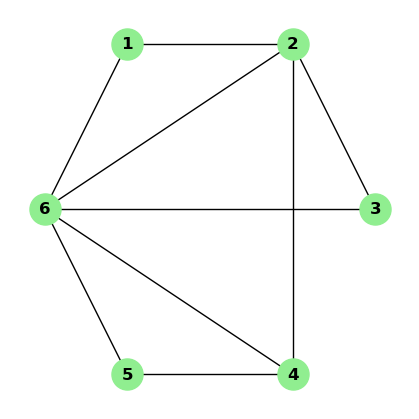
\includegraphics[width=2in]{undirected.png}
                \end{minipage}%
            \end{figure}

        \subsection*{e)}
            \begin{minipage}[t]{1\textwidth}
                Average degree of H: $c = \frac{2m}{n} = \frac{2(9)}{6} = \frac{18}{6} = \mathbf{3}$
            \end{minipage}%
            
        \subsection*{f)}
            \begin{minipage}[t]{1\textwidth}
                Density of H: $p = \frac{2m}{n(n-1)} = \frac{2(9)}{6(5)} = \frac{18}{30} = \mathbf{0.6}$
            \end{minipage}%
        
        \newpage
        \subsection*{g)}
            \begin{figure}[ht] % You can adjust the [ht] placement options
                \begin{minipage}[t]{0.5\textwidth}
                    \centering
                    \captionsetup{labelformat=empty} % Remove the label ("Figure 1:")
                    \caption{Complement of $H$, $H^{c}$:}
                    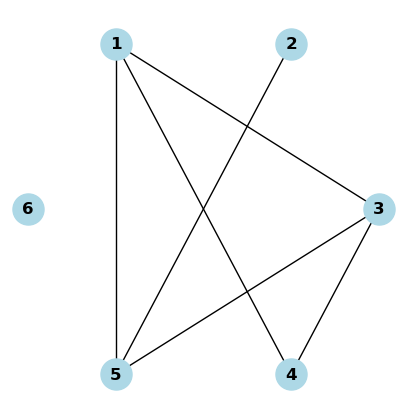
\includegraphics[width=2in]{undirected_complement.png}
                \end{minipage}%
            \end{figure}
    
    \section*{3.}
        \subsection*{a)}
            \begin{minipage}[t]{1\textwidth}
                $\mathbf{True}$. If a graph has 2 dominantating vertices, then every other vertex in the graph must
                have at the very least 2 adjacent vertices, namely, the two dominantating vertices. This means
                that it is impossible for a pendant vertex to exist in such a graph since a pendant vertex can
                can only have a single adjacent vertex.
            \end{minipage}
            \subsection*{b)}
            \begin{minipage}[t]{1\textwidth}
                $\mathbf{False}$. We can demonstrate that it is possible to draw a 4-regular graph on 7
                vertices with the following counter example:
            \end{minipage}
            \begin{figure}[ht] % You can adjust the [ht] placement options
                \begin{minipage}[t]{0.5\textwidth}
                    \centering
                    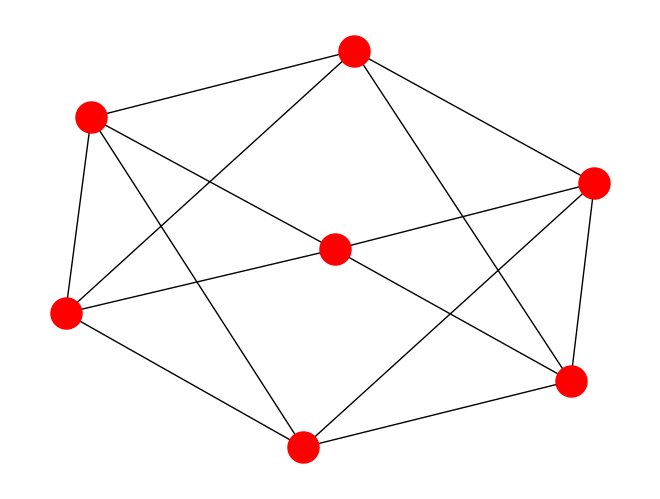
\includegraphics[width=2in]{four_regular.png}
                \end{minipage}%
            \end{figure}
            \subsection*{c)}
            \begin{minipage}[t]{1\textwidth}
                Only statement 3 is $\mathbf{True}$. This is beacuse every directed arch in the network
                simultaneously increases the total in-degree and total out-degree of the network by the
                same amount. Thus, counts for both attributes must always remain equal. 
            \end{minipage}

\end{document}